%%
%% Automatically generated file from DocOnce source
%% (https://github.com/hplgit/doconce/)
%%
%%


%-------------------- begin preamble ----------------------

\documentclass[%
oneside,                 % oneside: electronic viewing, twoside: printing
final,                   % draft: marks overfull hboxes, figures with paths
10pt]{article}

\listfiles               %  print all files needed to compile this document

\usepackage{relsize,makeidx,color,setspace,amsmath,amsfonts,amssymb}
\usepackage[table]{xcolor}
\usepackage{bm,ltablex,microtype}

\usepackage[pdftex]{graphicx}

\usepackage[T1]{fontenc}
%\usepackage[latin1]{inputenc}
\usepackage{ucs}
\usepackage[utf8x]{inputenc}

\usepackage{lmodern}         % Latin Modern fonts derived from Computer Modern

% Hyperlinks in PDF:
\definecolor{linkcolor}{rgb}{0,0,0.4}
\usepackage{hyperref}
\hypersetup{
    breaklinks=true,
    colorlinks=true,
    linkcolor=linkcolor,
    urlcolor=linkcolor,
    citecolor=black,
    filecolor=black,
    %filecolor=blue,
    pdfmenubar=true,
    pdftoolbar=true,
    bookmarksdepth=3   % Uncomment (and tweak) for PDF bookmarks with more levels than the TOC
    }
%\hyperbaseurl{}   % hyperlinks are relative to this root

\setcounter{tocdepth}{2}  % levels in table of contents

% Tricks for having figures close to where they are defined:
% 1. define less restrictive rules for where to put figures
\setcounter{topnumber}{2}
\setcounter{bottomnumber}{2}
\setcounter{totalnumber}{4}
\renewcommand{\topfraction}{0.95}
\renewcommand{\bottomfraction}{0.95}
\renewcommand{\textfraction}{0}
\renewcommand{\floatpagefraction}{0.75}
% floatpagefraction must always be less than topfraction!
% 2. ensure all figures are flushed before next section
\usepackage[section]{placeins}
% 3. enable begin{figure}[H] (often leads to ugly pagebreaks)
%\usepackage{float}\restylefloat{figure}

% prevent orhpans and widows
\clubpenalty = 10000
\widowpenalty = 10000

% --- end of standard preamble for documents ---


% insert custom LaTeX commands...

\raggedbottom
\makeindex
\usepackage[totoc]{idxlayout}   % for index in the toc
\usepackage[nottoc]{tocbibind}  % for references/bibliography in the toc

%-------------------- end preamble ----------------------

\begin{document}

% matching end for #ifdef PREAMBLE

\newcommand{\exercisesection}[1]{\subsection*{#1}}


% ------------------- main content ----------------------



% ----------------- title -------------------------

\thispagestyle{empty}

\begin{center}
{\LARGE\bf
\begin{spacing}{1.25}
Computing Across the Disciplines: Study Programs in Computational Science and Data Science
\end{spacing}
}
\end{center}

% ----------------- author(s) -------------------------

\begin{center}
{\bf A comprehensive path from undergraduate studies to graduate studies (Master and PhD levels) in Computational Science and Data Science at the University of Oslo }\\ [0mm]
\end{center}

\begin{center}
% List of all institutions:
\end{center}
    
% ----------------- end author(s) -------------------------

% --- begin date ---
\begin{center}
A whitepaper on how to organize Computational Science and Data Science initiatives at UiO, prepared for the Mat-Nat Fakultetet of the University of Oslo
\end{center}
% --- end date ---

\vspace{1cm}


\subsection*{Executive Summary}

This proposal seeks to transform the University of Oslo (UiO) to
become a leader nationally and
internationally in scientific discovery through large-scale
computations and data-driven research. The aim is to position UiO as a leader in
computational and data sciences by recruiting faculty whose expertise pertains
to large-scale computing and mathematical foundations of data science - both generalists (algorithm/tool developers) and specialists
(focused on specific disciplines).  

Scientific computing plays a central role in scientific investigations
and is central to innovation in most domains of our lives. It
underpins the majority of today's technological, economic and societal
feats. We have entered an era in which huge amounts of data offer
enormous opportunities, but only to those who are able to harness
them.  \href{{http://pathways.acm.org/executive-summary.html}}{By 2020, it is also expected that one out of every two jobs in
the STEM (Science, Technology, Engineering and Mathematics) fields
will be in computing}
(Association for Computing Machinery, 2013).

Furthermore, the \href{{http://www.economist.com/node/21553017}}{3rd Industrial Revolution} will alter significantly the demands on the workforce. To adapt a highly-qualified workforce to coming challenges  requires strong fundamental bases in STEM fields. Computational Science can provide such bases at all stages. Most of our students at both the undergraduate and the graduate level are unprepared to use computational modeling, data science, and high performance computing – skills valued by a very broad range of employers. The new department will also focus on the development of courses in computational science and data science tailored to the needs of the rest of society, both for the private and the public sector.

These developments, needs and future challenges, as well as
the developments which are now taking place within \href{{https://www.aps.org/publications/apsnews/201802/ostp.cfm?utm_source=APS+Physics+Main+Group&utm_campaign=fb7a2e7d6b-News+021218&utm_medium=email&utm_term=0_825303224b-fb7a2e7d6b-106513221}}{quantum computing, quantum information} and data driven discoveries (data analysis and machine learning) will play an essential role in shaping future technological developments. Most of these developments require true cross-disciplinary approaches, approaches which normally cannot be accomplished within the realms of one single disciplinary-based department. 


This document aims at developing strategies for meeting
these future challenges.  One important step in order to meet the
future, is the hiring of new researchers and faculty with the
competences and skills which are needed in order to harness the many
new possibilities, as well as developing new research and educational
strategies that can serve our society at large.




\vspace{6mm}

% inline figure
\centerline{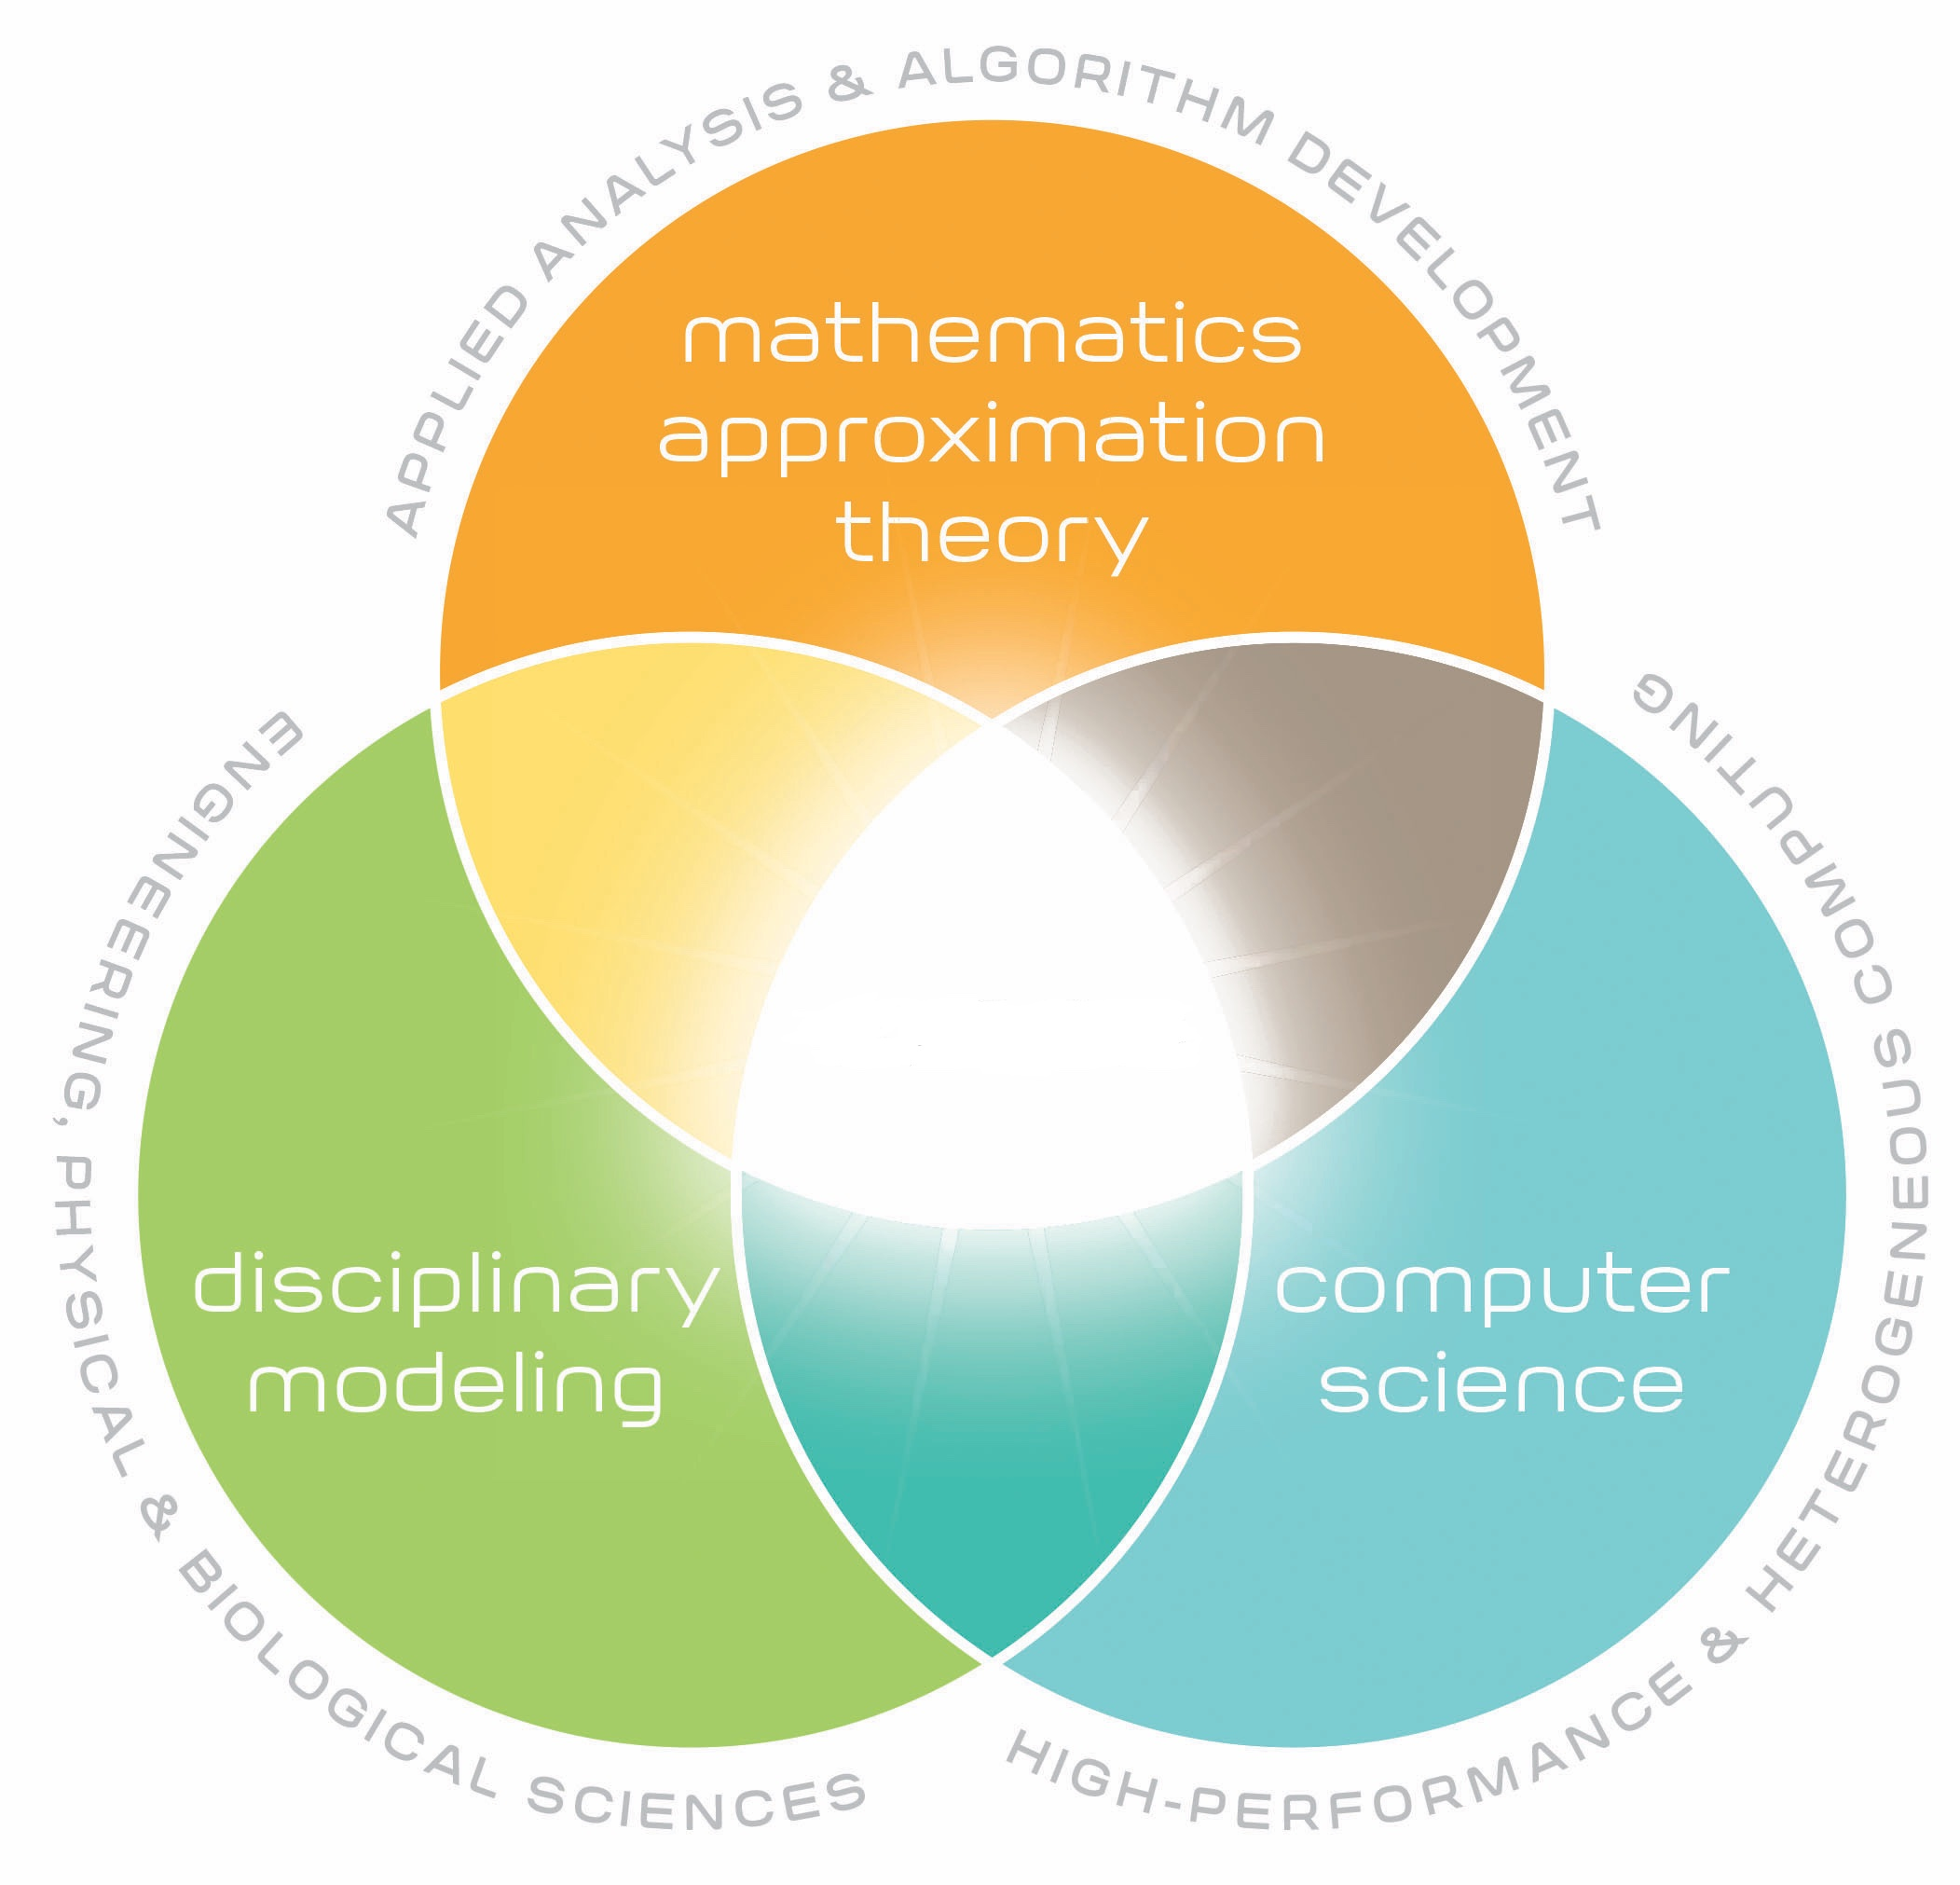
\includegraphics[width=0.7\linewidth]{figslides/cs.jpg}}

\vspace{6mm}



There are several possible ways to meet these challenges. The present document
focuses on the establishment of a new department (or possibly a center) on Computational and data Sciences. In Appendix A other organizational possibilities are presented without an in depth analysis. 

Irrespective of ways of organizing these activities, the university of
Oslo will need to hire at least some 25-30 new faculty in order to
meet future challenges. Many of the needed competences and research
area are only weakly covered, or are non-existing, by present faculty.

We propose thus a two-step process
\begin{itemize}
\item Establish a working group by April 1 2018. This working group  will be tasked to deliver a final report with various strategies  by the end of fall 2018.

\item From spring 2019, start the work needed to establish for example a new Department (or center), called \textbf{Department of Computational and Data Sciences} by fall 2020. The new department will be a hub for innovative thinking and pave the way for research and education in computational and data science across all disciplines. 
\end{itemize}

\noindent
The new department (or center) will be part of the
Matematisk Naturvitenskapelige Fakultetet (MNFak in brief) of the university of Oslo,
although it aims at becoming a true inter-disciplinary department
serving all colleges (Law, Natural Science and Mathematics, Medicine,
the Humanities, Education and the Social Sciences). It is the MNFak
which will propose to the board of the university of Oslo the
establishment of the department (eventually the center).  We propose thus
\begin{enumerate}
\item a new Department of Computational and Data Sciences (CDS) that is administered by the MNFak and meant to facilitate interdisciplinary science by fall 2020;

\item the injection of 25-30 new faculty  focusing on the science of computational modeling and data science;

\item the foundation for developing joint cutting-edge graduate and undergraduate programs. 
\end{enumerate}

\noindent
The new faculty will thus be tasked with developing new research and educational programs in Computational Science and Data Science. The hired faculty can/will have shared positions with existing departments (for example a 70\% position at the CDS department and 30\% at the department of Physics), similarly, faculty with a computational profile and interest at existing departments can have shared positions at the new department. This will ensure transfer of knowledge as well as the establishment of new and cross-disciplinary research and  oversee the development of new educational programs and efforts. 
A center solution cannot ensure the long-term sustainability of all these activities. A single department will also not be able to oversee the truly at large cross-disciplinary foundation of Computational Science and Data Science. 


These efforts will open doors to new scientific challenges,
will enable UiO to compete and propose new Center-level funding
opportunities as well as totally new research areas (in the Humanities for example) in computation and data-driven related 
areas that are currently beyond
our reach. It will facilitate the training of scientists and students to be an effective 21st century workforce.  It will also develop courses on modern computational techniques and data modeling that meet the needs of society, both for the public and the private sector. The metrics for
success are as follows. Within 5 years (2020-2025), we will have hired 25-30
world leading faculty that form the backbone of this
department, who will bring in single-PI grants and small-scale
(few-PI) collaborative grants, building the foundation for CDS to
develop large-scale funding. 

We have already developed (starting fall 2018) two new Master of
Science programs, one in \href{{http://www.uio.no/english/studies/programmes/computational-science-master/index.html}}{Computational Science} which includes almost all
disciplines at the MNFak and one on \href{{http://www.uio.no/english/studies/programmes/datascience-master/index.html}}{Data Science}.  These
programs form the basis for our educational efforts that will lead to
an \textbf{across the disciplines PhD program} serving the whole
university. The PhD program will start fall 2020 when the first
students from our two Master of Science program have finalized their
theses.  Based on the two exisiting MSc programs, the new department will research the possibilities of establishing similar MSc programs in Computation and Data Sciences for other disciplines.  Similarly, the new department will aim at establishing similar programs for outside users.  

The new department will coordinate many of its educational
activities with the newly established center of excellence in
education, the Center for Computing in Science Education. It will give
the Computing in Science Education initiative a formal institutional
basis  and together with the Center for Computing in Science Education it
will form a unique powerhouse in educational transformations. The new
department will

\begin{enumerate}
\item Develop a comprehensive set of courses and degree programs at both undergraduate and graduate levels that will give students across the university exposure to practical computational methods, understanding how to analyse data and more generally to the idea of computers as problem-solving tools. The department will also  develop  Software Carpentry and Data Carpentry courses. The courses and the degree programs can also be offered as intensive training courses and programs.	

\item Facilitate the adoption of computational tools and techniques for both research and education across campus, through education and faculty collaboration. A  department will facilitate the pursuit of these goals!	

\item Develop an all university PhD program in Computational Science and Data Science.

\item Based on the new programs (start fall 2018) on Computational Science and Data Sciece, Develop an all university Master of Science Program in Computational Science and Data Science.

\item Develop courses and course modules in Computational Science and Data Science for the private and the public sectors.

\item Develop a Master of Science program and a PhD program in Computational Science and Data Science tailored to the needs of the private and the public sectors, allowing for students residing outside UiO to develop their knowledge about Computational Science and Data Science.

\item Be a driving force in the education of  the next generation of school teachers and university teachers,  with a strong focus on digital competences. 
\end{enumerate}

\noindent
Finally, this department will facilitate the growth of the
university by participating in cross-cutting efforts such as the
upcoming life science initiative. Within 10 years, the
initiative will have secured Center-level funding via for example the Norwegian SFF system and the EU.
The department will also have fully developed  our graduate and undergraduate curriculae
with the addition of Bachelor’s programs in computational modeling and
data science, and will have strong enrollment numbers in all education programs. 


The new CDS department  will be unique among computational academic units nationally, the first to comprehensively
treat computation as the triple point of algorithm development and analysis, high performance
computing, and disciplinary knowledge with applications to scientific and engineering modeling
and data science. There is no such department in Norway and very few ones in Europe and Northern America. 
The above paradigm shift recognizes computation as a new discipline rather
than decomposed into isolated sub-disciplines, enabling application-driven computational
modeling and data-driven discoveries, while also exposing disciplinary computationalists to advanced tools and
techniques, which will ignite new transformational connections in research and
education. This research nexus also gives rise to the educational opportunities driven by similar
synergy, leveraging common resources among disciplines, and enabling joint programs and
unique degrees across the entire computational space.



\subsection*{Why should we focus on developing a department in Computational and Data Sciences?}

Modern problems in science and engineering bridge a vast range of temporal and spatial scales
and include a wide variety of physical processes. The analysis of such problems is not possible, so
one must turn to computation. To develop computational tools for such complex systems that
give physically meaningful insights requires a deep understanding of approximation theory, high
performance computing, and domain specific knowledge of the area one is modeling. National laboratories like \href{{https://www.simula.no/}}{SIMULA research lab} have addressed the interdisciplinary nature of computing by having experts
in numerical algorithms co-located with disciplinary experts who have a deep understanding of
computation, and who use scientific computing to address key topics in science.

The proposed organization with  algorithmic scientists and disciplinary scientists in STEM fields as well as other  fields is what facilitates the exploration of challenging multi-disciplinary and
interdisciplinary topics that could not otherwise be addressed. This key observation motivates
the model for the proposed department - a place where we will attack the critical problems
facing us in the 21st century, problem which require the development of computing skills across disciplines, from the traditional STEM fields to the Humanities, Law, Educational Science  and the Social Sciences. 
Furthermore, this department would strive to use
computing as a critical tool to explore fundamental scientific questions in subjects as diverse as
the physics of specific materials, evolutionary biology and data-driven economic forecasting. In addition, the synergy of data-driven computational
modeling, combining aspects of traditional scientific computing with data science and data
mining, is an exciting topic that this new unit will be uniquely suited to address. This is a rapidly
emerging field that touches many of the STEM disciplines but also Medicine, Education, the Humanities and the Social Sciences, and attracting world-leading talent in
this area is greatly facilitated by the introduction of the nurturing environment of the CDS department. Furthermore, the development of the Department of Computational and Data Sciences
has the potential to  catapult UiO into the position of being a
leader in this critical new field, and will open doors to new scientific challenges as well
as new Center-level funding opportunities.

To jump-start this new department at the ‘triple point’ of mathematics, computer science and
discipline-specific computation, we propose recruiting faculty who are experts in numerical
algorithms as well as those whose primary focus is the use of advanced computation to solve a
wide range of challenging scientific problems. 
Furthermore, we wish to define scientific projects where data-driven discovery can play a major role in future years.
In addition, we wish to recruit scientists - having
joint appointments with other units at UiO - whose expertise in computation on heterogeneous
and/or distributed computing platforms, such as hardware-accelerated computing (e.g., GPU
computing), cloud computing, and middleware for dynamic optimization across HPC
architectures. To provide a critical mass, we propose hiring 25 to 30 new faculty across the
aforementioned disciplines. Colocation and research and curriculum ties enable the CDS department  to
break down historical disciplinary boundaries, and become the synergistic leading-edge center
of computational activities on campus. Furthermore, colocating these scientists will enhance
the development of new computational algorithms to address pressing scientific and societal needs and
enable the creation and deployment of the robust numerical tools required for the pursuit of
leadership-class science in virtual laboratories.
Most importantly, the new department will enable new science through these unique interdisciplinary collaborations and will
become a focal point for computational research at UiO, bringing researchers in
computational and data sciences together with domain experts in astrophysics, bioinformatics, chemistry, geoscience
neuroscience, subatomic physics, materials science, life science, the Humanities, economy, Education  and many more.






\paragraph{Strengths, Possibilities and Synergies.}
The University of Oslo has within several of the STEM fields strong research and educational activities, exemplified through for example:
\begin{itemize}
\item Several Centers of excellence in research where Computational Science plays a major role

\item A newly established center of excellence in education research

\item Newly established Master of Science programs in Computational Science and Data Science

\item Several excellent groups in STEM fields that do Computational Science and Data Science

\item Computational topics are included in all undergraduate STEM programs, with the possibility to develop a bachelor program in Computational Science and Data Science for all university colleges

\item Several educational prizes and awards related to computational science 

\item Strong links with research laboratories like SIMULA research lab

\item UiO has the potential to develop cross-college educational programs in Computational Science and Data Science, from undergraduate programs to PhD programs that serve also the public and the private sectors

\item The courses to be developed can be offered to train employees and students outside UiO, serving thus the coming needs of for example Machine Learning for the public and the private sectors
\end{itemize}

\noindent
With a department (or center) we have the possibility to really position UiO as the leading Norwegian and perhaps European institution within Computational Science and Data Science.



\paragraph{Enhance Computational Science and Data Science across the disciplines.}
Data driven discovery and data driven modeling play already a central role in research. The global objective here is to strengthen and coordinate such activities by bringing together scientists and students across the disciplines.
UiO has already strong computational research and education activities within Mathematics and the Natural Sciences.
The aim here is to extend this to include

\begin{itemize}
\item Computational Science and Data Science in Mathematics and all of the physical sciences (Astrophysics, Chemistry, Geoscience and Physics)

\item Bioinformatics

\item Develop research programs in \href{{https://www.aps.org/publications/apsnews/201802/ostp.cfm?utm_source=APS+Physics+Main+Group&utm_campaign=fb7a2e7d6b-News+021218&utm_medium=email&utm_term=0_825303224b-fb7a2e7d6b-106513221}}{Quantum Computing and Quantum Information theory}. Many universities are now developing research and \href{{https://vprgs.msu.edu/event/interdisciplinary-forum-quantum-information-science}}{educational strategies in Quantum Computing}

\item Develop data-driven discovery research programs utilizing recent developments in machine learning

\item Computational life science

\item Computational Materials Science

\item Computational Economy and Data Science and computing in Law and the Social Sciences

\item Data Science and computing in the Humanities
\end{itemize}

\noindent
The new department will host and coordinate research and educational programs in Computational Science and Data Science. In particular research and education that involve  data analysis and Machine Learning will play a central role here. Similarly, the new department will be responsible for developments in quantum computing and quantum information theories. 

\subsection*{Courses and degree programs}

Creation of a robust, coherent set of undergraduate and graduate degrees, with accompanying
courses, supports two complementary goals. First, a coherent program will allow the university
to consolidate undergraduate and graduate training in computation in the STEM fields as well as introducing computing to other disciplines, reducing
redundancy in the courses taught and allowing the university to offer a wider range of more
specialized advanced courses. Second, we will create a robust set of degrees that are designed to give our 
students a strong introduction to computing
that will complement UiO’s existing disciplinary training, and which will make them better suited
to be a part of the workforce in the 21st century, but also to be able to develop and use computing and data Science across the disciplines. These programs will include:
\begin{enumerate}
\item An undergraduate program in Computational and Data Sciences tailored to various disciplines.

\item We have already (from fall 2018) two new Master of Science programs in Computational Science and Data Science dailored to STEM fields. The aim is to extend these to other colleges.

\item Develop a cross-college PhD program in Computational Science and Data Science.

\item Develop courses and course modules in Computational Science and Data Science for the private and the public sectors.

\item Develop a Master of Science program and a PhD program in Computational Science and Data Science tailored to the needs of the private and the public sectors, allowing for participants residing outside UiO to develop their knowledge about Computational Science and Data Science.

\item Be a driving force in the education of  the next generation of school teachers and university teachers,  with a strong focus on digital competences. 
\end{enumerate}

\noindent
This range of options will allow some number of students to dive deeply into
computation through the degree programs, and will enable a much broader swath of the UiO
population to learn about some aspects of computational and data science through not only the various programs but also through the courses to be developed by the new department. 

One desired result of the creation of these
courses and programs is the foundation of a strong community of students from different
disciplines who use similar techniques to solve a wide range of problems, which will promote
broad, interdisciplinary thinking and will help to raise the visibility of computing throughout the UiO campus. We note that an extra benefit of these educational
efforts is that UiO will become an ideal place to perform research in computational science
education, a topic of critical importance that has thus far received little scholarly attention. The new department will have strong links with the recently established Center for Computing in Science Education. 




\paragraph{Long term goals and sustainability.}
The overall goal of this department is to bring together world-leading
faculty who combine the most important aspects of computation and
disciplinary research, thus enabling cutting-edge interdisciplinary
science and the training of both undergraduate and graduate
students. The department will be economically sustained through the standard base
university funding, as any other department at Norwegian universities. 
However, additional funds will be
realized by the securing for example Center-level funding (as well as many
single- or few-PI grants), as well grants obtained the PIs that sustain graduate
students, post-docs, travel and other associated expenses.  In order
to ensure the success of these efforts, the proposed department must
be financially sustainable. Basic university funding (beyond faculty
and support staff salaries) is necessary to support fellowships for
top graduate students, speaker series and honoraria, visitor support,
hardware purchases, and startup packages.

The enclosed appendices contain more details about the structure of
the planned department, with research and education plans. Links to
similar and recently established departments are also presented.






\subsection*{Appendix A: Tentative list of   working group members (February 2018)}


\begin{enumerate}
\item Bioscience: \href{{http://www.mn.uio.no/ibv/english/people/aca/tomand/}}{Tom Andersen}, \href{{http://www.mn.uio.no/ibv/english/people/aca/mariafy/}}{Marianne Fyhn} and \href{{http://www.mn.uio.no/cees/english/people/technical/alexajo/}}{Lex Nederbragt}

\item Chemistry and Hylleraas Center for Quantum Molecular Sciences: \href{{https://www.mn.uio.no/kjemi/english/people/aca/michelec/}}{Michele Cascella}

\item Geoscience: \href{{http://www.mn.uio.no/geo/english/people/aca/geohyd/johnbur/index.html}}{John Burkhart}, \href{{http://www.mn.uio.no/geo/english/people/aca/metos/josepl/}}{Joe Lacasce} and \href{{http://www.mn.uio.no/geo/english/people/aca/geohyd/thomasc/}}{Thomas Vikhamar Schuler}
% o IFI Bioinformatics: Torbjørn Rognes and Geir Kjetil Sandve

\item IFI: \href{{https://www.mn.uio.no/ifi/personer/vit/andrea/}}{Andreas Austeng},\href{{http://www.mn.uio.no/ifi/personer/vit/xingca/index.html}}{Xing Cai}, \href{{http://www.mn.uio.no/ifi/english/people/aca/sundnes/index.html}}{Joakim Sundnes}

\item Math: \href{{https://folk.uio.no/kent-and/}}{Kent-Andre Mardal} and \href{{http://www.mn.uio.no/math/personer/vit/knutm/index.html}}{Knut Mørken}

\item Physics and Center of Computing in Science Education: \href{{http://www.mn.uio.no/fysikk/english/people/johnmai/}}{John Mark Aiken}, \href{{http://mhjgit.github.io/info/doc/web/}}{Morten Hjorth-Jensen} and  \href{{http://www.mn.uio.no/fysikk/english/people/aca/malthe/}}{Anders Malthe-Sørenssen}

\item SIMULA research lab: \href{{http://www.mn.uio.no/ifi/personer/vit/xingca/index.html}}{Xing Cai}, \href{{https://www.simula.no/people/simon}}{Simon Funke}, \href{{https://marierognes.org/}}{Marie Rognes}, \href{{http://www.mn.uio.no/ifi/english/people/aca/sundnes/index.html}}{Joakim Sundnes}, and \href{{https://www.simula.no/people/aslak}}{Aslak Tveito}
% o Economy: Kjetil Storsletten and Halvor Mehlum? Tentative

\item Department of Political Science: \href{{http://www.sv.uio.no/isv/personer/vit/bjornkho/}}{Bjørn Høyland}

\item Department of Sociology and Human Geography: \href{{http://www.sv.uio.no/iss/english/people/aca/torkildl/}}{Torkild Hovde Lyngstad}

\item Department of Psychology: \href{{http://www.sv.uio.no/psi/english/people/aca/nikolaic/index.html}}{Nikolai Olavi Czajkowski}
\end{enumerate}

\noindent
\paragraph{Summary of Timeline.}
\begin{enumerate}
\item Establish a working group by April 1 2018. The working group will be tasked with evaluating various scenarios for strengthening Computational Science and Data Science at UiO. The report will be finalized during Fall 2018.

\item Start establish from spring 2019 a department (or possible center)  called \textbf{Department of Computational and Data Sciences}, with inauguration by end of 2020/begin 2021. 

\item \href{{http://www.uio.no/english/studies/programmes/computational-science-master/index.html}}{New Master of Science Program on Computational Science starts fall 2018}

\item \href{{http://www.uio.no/english/studies/programmes/datascience-master/index.html}}{New Master of Science Program on Data Science starts fall 2018}

\item Establish  a cross-college PhD program in Computational and Data Sciences, start fall 2020. This PhD program will be a collaboration between the Natural Sciences, Humanities, Social Sciences, Medicine and Education. 

\item Develop a corresponding cross-college MSc program in Computational Science and Data Science by fall 2020.

\item An undergraduate program in Computational and Data Sciences tailored to various disciplines by fall 2020

\item Develop courses and course modules in Computational Science and Data Science for the private and the public sectors by fall 2019.

\item Develop a Master of Science program and a PhD program in Computational Science and Data Science tailored to the needs of the private and the public sectors, allowing for students residing outside UiO to develop their knowledge about Computational Science and Data Science by fall 2021.

\item Submit an application called \textbf{Computing Across the Disciplines} for a Marie Curie training network by spring 2019, 15 PhD positions
\end{enumerate}

\noindent
\paragraph{Alternative paths to be explored.}
The present version of the document focuses on the establishment of a new department. 

Other possibilities that should be explored are: 
\begin{enumerate}
\item The establishment of one or more centers in Computational Science and Data Science. The center(s) will lay the foundation for cross-disciplinary activities and establish the necessary foundations and preparations for launching for example a new department. It will develop research projects across disciplines as well as develop educational programs and initatives related to the establishment of an eventual new department or modification of existing departments.

\item A cluster hire at various departments in order to strengthen overall research and educational competences in computational science and data science. In this case one would most likely need a center or department  that coordinates such activities. Here one could think of for example 3-5 new positions in Computational Mathematics at the Department of Mathematics, a similar amount in Physics, Bioscience, Geoscience, Economy, Social Science etc.;

\item The enlargement/change/extension of existing departments. As an example, the present Department of Mathematics could be enlarged in order to accomodate the future needs. 
\end{enumerate}

\noindent
\subsection*{Appendix B: Structure and Justification for Planned Organization}

We envision that the CDS department  will be a truly interdisciplinary unit that strives to focus on algorithmic
science and its applications to a range of critical research topics. The CDS department will consist of 25-30
faculty, comprising generalists and disciplinary scientists. The generalists develop cross-disciplinary
tools addressing large classes of problems. The disciplinary scientists pursue
model/algorithm development from a domain-specific perspective, enabling application-specific
approximations and optimization of performance on exascale problems. The nexus of these
groups is what makes CDS unique.

The cross-disciplinary  working group  that developed this
proposal seeks the creation of a joint, inter-college department as the ideal solution. This
structure, is necessary to facilitate the recruiting of a core
group of faculty whose focus is on algorithmic science that can be applied to new scientific
challenges and computational platforms. The reasoning behind this is straightforward - the
fundamental science we are interested in developing is clearly
growing beyond the boundaries of existing STEM disciplines, in the same way that the discipline
of computer science grew beyond the boundaries of historical roots in mathematics or electrical
engineering. It is advantageous to be at the forefront of this trend.
This new department is at the forefront of a key paradigm shift. Discipline-focused departments
tend to only place value on the new science a computer programs can explore, and to not place
value on the time or energy it takes to develop critical algorithms and tools that provide a deeper
understanding of fundamental processes in the various disciplines. By placing the 
home of computational scientists in this new department, we accomplish two critical goals.
First, a single department focused on the science of computation will strengthen the goal of
interdisciplinary collaboration, as faculty in this new unit will have a wide range of backgrounds
in many traditional disciplines, and not only the traditional STEM disciplines. Second, the new department will break down traditional
barriers between departments, as the
common theme of the new department is the science of algorithms and their applications, providing a key place for critical interactions between
different scientific communities.
While many faculty will have full appointments in the department, joint appointments will help to
cement interdepartmental collaboration and build up a strong interdisciplinary community. This
gives UiO the flexibility to grow into this critical area by hiring cutting-edge interdisciplinary
scientists, and will also allow existing disciplinary departments the opportunity to grow beyond
their current boundaries. 

The joint appointments with other departments will play an important role in cementing the structure of the CDS department, strengthening cross-disciplinarity collaborations. Furthermore, the task of developing new and joint courses will require extensive collaborations across departments. As an example, faculty hired by the new department could have a 70\% appointment with the new department and 30\% with a single discipline oriented department. Similarly, a researcher with linked to the department of Chemistry, could have a shared position of for example  20\% at the CSD and 80\% at the department of  Chemistry. These joint appointments will facilitate the seeding of new research and the development of new courses and degree programs. 

One can view the new department as a hub which focuses on Algorithms, Computing, Big Data, Mathematics, Quantum Computing, Machine Learning and Statistical Analysis in close collaboration with scientists working from the Physical Sciences (Chemistry, Astrophysics, Physics, Geoscience, Mechanics, Materials Science), Life Science (Bioscience and Medicine), Law, Education, Social Sciences and the Humanities. The new department will develop and strengthen the field of Computational Science and Data Science in close collaboration with all involved departments (from the MNfak and other colleges), increasing thereby the overall general competences of our students and scientific staff on these topics. 
The following figure illustrates schematically these links, with the two inner circles representing the most likely key research activities of the new department. 



\vspace{6mm}

% inline figure
\centerline{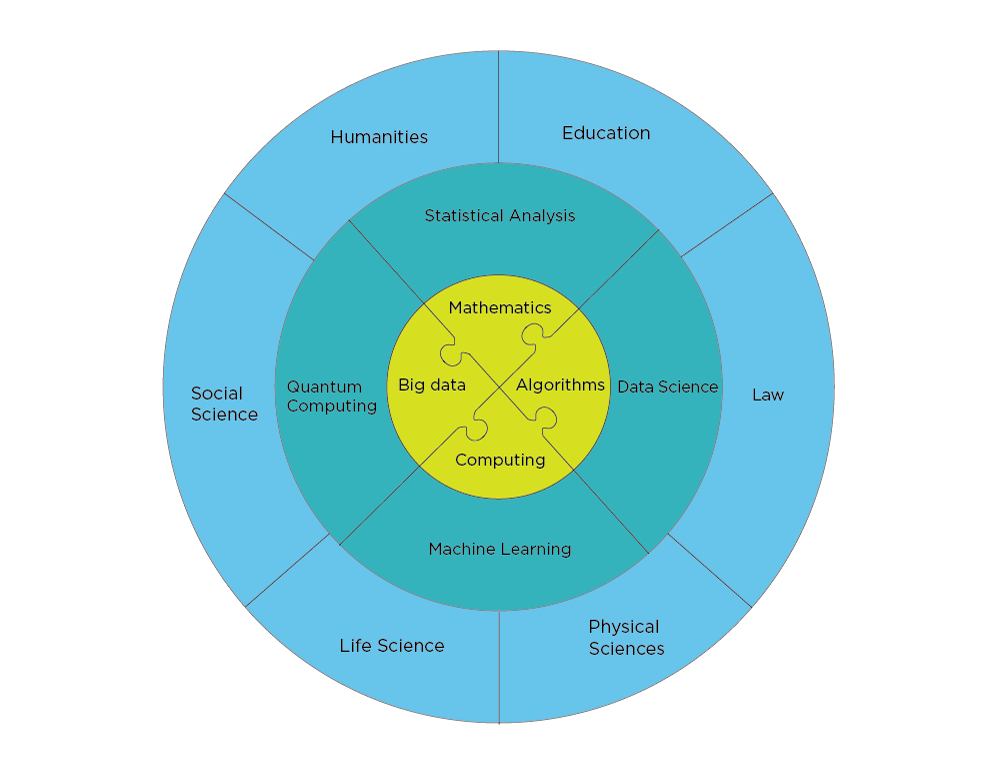
\includegraphics[width=1.0\linewidth]{figslides/topics.png}}

\vspace{6mm}



\paragraph{Funding.}
In order to secure funding in addition to those guaranteed by the University and the ministry of education and research, the department will seek assiduously center funding  from the Norwegian SFF and SFI system (under the auspices of the Research Council of Norway) as well as similar funding possibilities  from the EU. In addition, we expect the faculty to bring in regular research grants either from industry, the Research Council of Norway or the EU. 

We aim also at exploring and having, out of the 25-30 positions, five positions at the level of associate or full professor as endowed chairs and professorships from the private sector. We will in particular target companies where computational science and data science will play a major role in the future. The design of research projects linked to the needs of these companies as well as the PhD and Master of Science programs discussed below, will make sure that both the private and the public sector will benefit from highly qualified candidates.  

Below we discuss several  possible research directions where  faculty hires can start new research directions, in close collaborations with specialists from various departments.


\subsection*{Appendix C:  Sampling of new and transformational science that will  be enabled by the new department}

There are several new and emerging research directions where the new department will play and can play a major role. 


\paragraph{Computational life science.}
The Life Sciences is transforming with the explosion of
High-throughput data generation technologies and the need for
integrating these across all the levels of the biological hierarchy. A
'system-dynamic' (Systems Biology) approach will dominate research in
the coming decades. Here, computational modelling to integrate the
various data types and data sets will be a driving force. Similar
developments are seen in the field of molecular image analysis, where
computational methods to integrate the image streams will become
essential to make sense of the growing amount of data. Translational
Bioinformatics, bridging the gap between the laboratory, computer and
the clinic, with the ultimate goal of personalised medicine, is an
important, and exciting new dimension. Many of these developments
require cross-disciplinary thinking, and often breakthroughs in
Bioinformatics/Computational Life Science start with creatively
adjusting and implementing algorithmic or computational solutions
originally developed for other fields. A CDS department that has
multidisciplinarity as its founding principle, and brings
computationally skilled researchers from many fields together, will
provide a solid foundation for researchers working towards these
developments.



\paragraph{Develop data-driven discovery research programs utilizing recent developments in machine learning.}
 \textbf{Machine Learning} plays nowadays a central role in the analysis of
large data sets in order to extract information about complicated
correlations. This information is often difficult to obtain with
traditional methods. For example, there are about one trillion web
pages; more than one hour of video is uploaded to YouTube every
second, amounting to 10 years of content every day; the genomes of
1000s of people, each of which has a length of $3.0\times 10^9$ base
pairs, have been sequenced by various labs and so on. This deluge of
data calls for automated methods of data analysis, which is exactly
what machine learning provides.  Developing activities in these
frontier computational technologies is thus of strategic importance
for our capability to address future science problems. The
applicability of big data, data-driven discoveries, data-driven
modeling and machine learning covers basically all disciplines and
fields, with applications spanning from materials science, mechanics,
medicine, applied mathematics, economic forecasting etc. Machine
learning and big data concepts are being exploited in more and more
fields.  The big data challenge will be in the forefront of biology
and life science research in the next few years.  In materials science
machine learning allows us to parametrize results from quantum
mechanical calculations in terms of classical interactions. These
interactions are in turn suitable for large scale molecular dynamics
simulations of complicated systems spanning from subatomic physics to
materials science and life science.  To develop a multiscale science
program starting with the smallest constituents and moving to larger
systems can most likely only be done with the development and
application of machine learning algorithms.  Economists and policy
makers need up-to-date information on the state of the economy to
formulate effective policies. Variables such as GDP, Gini factors,
unemployment rates, quality of life data etc are normally used as key
indicators. These data are often only available with delays between
collection and availiability to analysts, making it thus difficult to
asses properly their relevance. Machine learning algorithms have the
potential to deliver improved predictions as well as correlations and
proper error estimates. The examples discussed here represent just a
few of the possible applications of Machine Learning algorithms that
the new department can aid in developing. To develop these research
lines will be achieved most effectively within the multidisciplinary
CDS department.


\paragraph{Develop research programs in Quantum Computing and Quantum Information theory.}
Enabling simulations of large-scale quantal many-particle systems is a
long-standing problem in scientific computing.  Quantum many-particle
interactions define the structure of the universe, from nucleons and
nuclei, to atoms, molecules, and even stars. Since the discovery of
quantum mechanics, a lot of progress has been made in understanding
the dynamics of certain many-particle systems. While some of our
insight comes from a small set of analytically solvable models,
numerical simulations have become a mainstay in our understanding of
many-particle dynamics. The progress in numerical simulations has
accelerated in the last few decades with the advent of modern high
performance computing (HPC) and clever developments in classical
simulation algorithms such as, quantum Monte Carlo,large-scale
diagonalization approaches, Coupled-Cluster theory and other
renormalization schemes.  Despite the monumental advances, classical
simulation techniques are reaching fundamental limits in terms of the
size of the quantum systems that can be processed. Fortunately, the
disruptive new field of quantum simulations has emerged, promising to
enable simulations far beyond those which are classically
tractable. In particular, scientific applications concerned with
simulations of interacting fermions on a lattice are poised to reap
the benefits of quantum simulations.  Mathematical models of
interacting fermions naturally extend to describe vastly different
physics such as that of correlated electronic and the correlated
nuclear systems.

 Recent progress in quantum computing as well as digital and analog
Quantum Algorithms (QAs) promise to enable the exciting possibility of
performing simulations that are beyond the reach of all existing and
future classical supercomputers. Despite the progress, there is still
a gap between the resources required by state-of-the-art QA and the
resources offered by available and near-future quantum hardware. It
may take decades of quantum hardware development and engineering
before the current QAs will outperform classical exascale class
simulations. Therefore, to impact scientific computing on a more
relevant time scale, improving the scalability and efficiency of
quantum simulation algorithms is of the highest
importance. Developments in quantum information algorithms and their
mathematical properties, as well as their applications will play a
critical role in studies of relevance for a wide variety of fields,
from the design and studies of new materials to our basic
understanding of systems of interest in chemistry and physics. The new
department, in close collaboration with disciplinary experts, can play
an essential role in developing this field by hiring world-leading
experts in quantum information theory and quantum computing.

\paragraph{Computational Social Science.}
Survey data, the engine of the behavioral revolution of the social sciences is about to run its course, with low response rate and poorly representative samples being the norm rather than the exception.  Fortunately, vast amount of new information from social media, via digitalized governmental archives, to population registries are opening up new exiting avenues for innovative social science research, such as paternity leave and children’s performance in school, extent of censorship in Chinese online new reporting, or conditions for receptiveness to fake news. Moreover, the new data availability in combination with tools from machine-learning has spurred an interest in prediction and sophisticated policy-recommendations, ranging from optimize relocation of immigrants given their skill-set and local labor market needs, via probabilistic detection of election fraud, to forecasting of popular unrest and civil war. The undertaking of such research questions was, until recently, outside the realm of social science. There are however limits to the amount of new insights that can be obtained purely from richer data and “black-box” import of machine-learning tools. More robust, new insights require similar steps to be taken in the development of applied, testable, theoretical models to facilitate direct empirical evaluations of the model dynamics and the consistency of the model with the data. Such a step requires a solid grounding in computing.



\paragraph{Computational Geoscience.}
Geoscience has long been a computationally-intensive area. A typical
climate simulation, used for example in the future projections
discussed by the Intergovernmental Panel on Climate Change (IPCC), can
generate a petabyte (1 million gigabytes) of data. Weather forecasts
involve suites of complex simulations, which are then averaged to
assess the probability of different scenarios. These models simulate
not only the atmosphere, but the important interactions with the
ocean, land and vegetation. Sophisticated models are also used for
studying tectonic continental shifts, to understand the geology and
climate of previous epochs, thereby informing our understanding of
prehistoric life. And similar models are used to simulate hydrological
reservoirs and the melting occurring at the base of major
glaciers. Computation is so central to the geosciences that it is
impossible to imagine the study without it.

The computational approaches relevant for geoscience can be grouped in
two classes: simulation and analysis. Geoscientific computation
demands advance programming techniques and optimized simulations, to
ensure the fast calculations. Changes in the global ocean circulation
can take tens of thousands of years, demanding the most rapid
simulations possible. High performance computing approaches, for
example using graphical processing units (GPUs), are now being applied
to climate models, greatly increasing performance.  The large amount
of data generated by geophysical simulations is also a challenge and
is well-suited for big data techniques. Machine learning is beginning
to be used in weather forecasting and in climate simulations. This has
led to the identification of weather patterns missed by researchers
and to the identification of extreme events like cyclones and
“atmospheric rivers”, on par with that of human
analysts. Computational geoscience is an exciting and developing
field, and one which will make major inroads to the earth sciences in
the future.

\paragraph{Computational Psychology.}
Large files of audio/video are currently unused since data is in a
form that is unavailable for quantitative analysis (such as video of
weekly clinical interviews from multi-center trials of treatment for
thousands of patients). Analysis of prosody can shed light on change
processes, and should automatic transcription reach a sufficiently
good level, this will, in combination with natural language
processing, open up many interesting research questions.

Accumulated data from online use already provides measurements of
quantities such as personality, attitudes, skills or mental disorders
which in many cases have proven to approach the level of the best
instruments we have. Here one obtain much more, especially since
clinical treatment will increasingly be supplemented by electronic
registrations in the future, as well as being able to disconnect data
from sensors in smart devices. Present instruments in use generate
relatively large amounts of data (from for example EEG, ERP, and fMRI), and newer
methods of pattern recognition/classification can shed light on a
number of research questions.

\paragraph{Machine learning in education research.}
Quantitative education research has historically been done at the
micro-scale (classrooms) and the macro-scale (K-12, baccalaureate
degree programs, etc.). Micro-scale research has been done using
traditional correlational statistics with data gathered from surveys,
conceptual tests, classroom observations, etc. With the advent of the
\emph{digital classroom} student behavior can now be examined in fine
grain. Students access of online homework platforms, video lectures,
and interactions with peers via online course forums has created new
data sources for education researchers. New technologies such as
computer textual analysis can pick apart student conceptual
understanding of hard concepts in science and mathematics. Intelligent
tutors can provide real time feedback to students as they solve
problems. At the macro-scale students’ career decisions within their
programs can be modeled. What courses they choose to take, who they
choose to take courses from, and their comments on said courses, form
new data sets which can be used to predict student decisions and
provide timely feedback to students and faculty advisers. Ultimately
these data sets can form a high dimensional picture of student
learning painted by machine learning.


\subsection*{Appendix D:  Outline of degree programs and courses}

This appendix summarizes the set of degree programs and courses that
can/should be administered by the new department. The range of
offerings gives students the opportunity to engage with computational
science at a variety of levels, from single courses to graduate
programs. Market research and feedback from employers indicate that
engaging with one or more of the proposed programs will substantially
enhance the student's career prospects. The new classes will move to
the new department once the department opens ist doors.

\paragraph{Degree programs.}
The MNFak  offers from fall 2018 two new programs at the Master of Science level in Computational Science and Data Science. These programs are
\begin{enumerate}
\item \href{{http://www.uio.no/english/studies/programmes/computational-science-master/index.html}}{Computational Science}, start fall 2018

\item \href{{http://www.uio.no/english/studies/programmes/datascience-master/index.html}}{Data Science}, start fall 2018

\item Develop similar Master of Science programs tailored to other colleges at UiO, including the Humanities, Law, the Socials Sciences, Medicine and Education by fall 2020

\item Develop an all university PhD program in Computational Science and Data Science by fall 2020

\item Based on these programs and the gained experiences we plan to develop a Master of Science program in Computational Science and Data Science tailored to the needs of the private and the public sectors. This will allow students residing outside UiO to develop their knowledge about Computational Science and Data Science by fall 2021

\item Develop a PhD program in Computational Science and Data Science tailored to the needs of the public and the private sectors (so-called nærings PhD in Norwegian)

\item Develop a bachelor program in Computational Science and Data Science by 2021
\end{enumerate}

\noindent
The Master of Science and PhD programs that will target students from outside UiO (from partner companies, public and private sectors)
will be developed in close collaboration with external stake holders. 

\paragraph{Courses.}
There are several existing and planned courses which could be offered by the new department.
These are
\begin{enumerate}
\item FYS-STK4155 Applied Data Analysis and Machine Learning  (first time fall 2018)

\item IN4230 High-Performance Computing  (first time spring 2019)

\item MAT4110 Computational Mathematics

\item FYS4150 Computational Physics

\item New courses on advanced data analysis and machine learning including for example
\begin{itemize}

  \item Supervised and unsupervised machine learning

  \item Data analysis and machine learning tailored to the Humanities

  \item Data analysis and machine learning tailored to the Social Sciences

  \item Data analysis and machine learning applied to Education programs

  \item Data analysis and machine learning applied to Law 

\end{itemize}

\noindent
\item Multi-particle methods for the Physical Sciences and Life Science

\item Courses on quantum computing and quantum information theory

\item Courses on computations in economy

\item Courses on software carpentry and data carpentry

\item ....
\end{enumerate}

\noindent
Many of these courses, if properly modularized, can be offered as intensive training courses and programs. In particular, such courses will be attractive for both the private and public sectors. The following courses could be offered
\begin{enumerate}
\item Introductory Scientific Python

\item Advanced Scientific Python

\item Data Science and visualization

\item Applied numerical mathematics

\item Computational finance

\item Big data graph analysis

\item Supervised machine learning with scikit-learn and TensorFlow

\item Unsupervised machine learning with scikit-learn

\item Data-driven entrepreneurship

\item Courses tailored to the needs of specific companies

\item and more specialized modules
\end{enumerate}

\noindent
\subsection*{Appendix F: Examples of Centers and Departments other places}


In Norway it is only UiO which offers a Master of Science program on Computational Science and Data Science. All other universities have only Master of Science programs on Computer Science. The University of Bergen has a Master of Science  program on Applied Mathematics while UMB has only a Master of Science on Bioinformatics and Data analysis. These are limited and more focused programs. Nationally, UiO is the only university which offers broad programs in Computational Science and Data Science. 
The goal in Oslo is to establish a department which covers both Computational Science and Data Science across colleges and disciplines. The department will be responsible for these educational programs and oversee that a coherent and modern selection of courses is offered and developed. The courses should reflect the needs of society at large as well as the specific research projects.  This will give UiO a unique position in Norway. 

Out of 95 universities polled in the USA, there are less than 15 which have a department on Scientific Computing
and more than 50 that have a center on Scientific Computing. Between 20 to 30 of these offer a bachelor, Master of Science or PhD program. On Data Science there are approximately 30 departments and 40 centers. Almost 50 of these universities offer a Masters degree in Data Science and close to 40 a PhD in Data Science. 
An excellent example of a department which includes computational science and data science is the newly established \href{{https://cmse.msu.edu/}}{department at Michigan State University}.

For the department of Michigan State University, the process which led to the establishment of the new department started fall 2013 and the new department opened its doors in fall 2015. It counts now 31 faculty of which 24 of them have shared positions with other departments. It offers a series of courses at all levels, minors and majors in Computational Science as well as its own graduate program. The department offers also a dual PhD with other departments. This option has been particularly popular with Physics students.

The new hires cover most STEM fields and the department has been central in starting new cross-disciplinary research activities. There are strong activities in life science and bioinformatics as well as in statistics, mathematics, physics, geoscience  and engineering. This department can serve as a role model for the development of a similar department at UiO. 

Other departments with similar scope and programs  in Northern America are (the list is not exhaustive)
\begin{enumerate}
\item \href{{https://www.cse.gatech.edu/}}{School of Computational Science and Engineering at Georgia Institute of Technology}

\item \href{{https://cse.ucsb.edu/}}{Computational Science and Engineering at University of California Santa Barbara}

\item \href{{http://www.ncat.edu/coe/departments/cse/index.html}}{Computational Science and Engineering at North Carolina Agricultural and Tecnological State University}

\item \href{{https://cse.illinois.edu/}}{Computational Science and Engineering at University of Illinois Urbana-Champaign}

\item \href{{https://www.sc.fsu.edu/}}{Department of Scientific Computing at Florida State University}

\item \href{{https://datascience.nyu.edu}}{New York University} 
\end{enumerate}

\noindent
Most of the other university in Northern America have a typical department of Computer Science. Programs in Computational Science and Data Science are frequently offered by the department of Mathematics and/or the department of Computer Science.
\begin{enumerate}
\item Purdue CCAM (Center for Computational {\&} Applied Mathematics)
\end{enumerate}

\noindent
At the time of writing, no such poll has been made for European universities. From the list over Masters programs, the countries with the largest focus on these topics are Germany (\href{{http://www.simtech.uni-stuttgart.de/}}{SimTech in Stuttgart is a good example}), Sweden and Switzerland. 
Examples of interest in Europe are the 
\begin{itemize}
\item \href{{http://www.lse.ac.uk/seds/}}{London School of Economics}

\item \href{{http://www.imperial.ac.uk/quantitative-sciences-institute/about}}{Imperial College and its Quantitive Sciences Research Institute}

\item \href{{https://www.ics.usi.ch/}}{Swiss Institute of Computational Science}
\end{itemize}

\noindent
while in Austria we have the 
\begin{itemize}
\item \href{{http://www.csc.univie.ac.at/ik/}}{Vienna Graduate School in Computational Science}
\end{itemize}

\noindent
The Society for Industrial and Applied Mathematics (SIAM) \href{{https://www.siam.org/students/resources/cse_programs.php}}{keeps track of graduate programs in computational Science}. The list is most likely not complete. 

In addition to the traction seen within data driven discoveries,
Quantum Information Science (QIS) is also gaining considerable
momentum presently. 
This represents a truly cross-disciplinary activity that cannot be placed within one single
department.
Though the disruptive potential of QIS has been
known for over 20 years, it has been in a nascent state with a number
of academic, industrial and government groups striving to understand
the basics physics and to build and control many-qubit systems.
There has been steady progress to a tipping point where the
realization of practical QIS systems is imminent; for example
the leading group in the field (Google Quantum AI) recently argued
that small-scale commercialization of quantum computing devices is
expected within 5 years; moreover quantum chemistry may be a
“killer app” for small quantum computing systems; and prototype
demonstrations are already emerging.  IBM is providing a 20 QUBIT
system for public use, and they expect to deliver a 50 QUBIT system in
the near future.

Strategic partnerships are developing between universities, large
corporations, startups, as well as federal and private funding
agencies in the USA.  Some of the major industrial and government investors are
Google, IBM and Microsoft. In the USA both the Department of Energy 
and the National Science Foundation are developing 
QIS programs with several new initiatives.


\begin{itemize}
\item In the second paragraph, "these future challenges" can perhaps be
\end{itemize}

\noindent
explained better. (It was only argued that computational science
and data science are important.) How about moving some of the
texts from section "Why should we focus on developing a
department in Com- putational and Data Sciences?"



% ------------------- end of main content ---------------

\end{document}

